\chapter*{10) Evaluation of Object-Oriented Design Patterns in Game Development}

  \section*{Introduction}
    The game industry has been considered to produce revenue greater than the movie industry and its development rate has been one of the most fast growing in the USs economy. Furthermore, game design and the methods used for easier and more efficient development constitute a very interesting open research field. Futhermore, games are the first and somtimes the only market for advanced graphics techniques to demonstrate the quality of graphics they produce. The distinction between games and other forms of software is that, in games, the development groups consist of people with different field of expertise (scripters, designers, programmers, musicians, graphic artists and testers). A speculation about the absence of scientific reaserch is that games are widley considered a ``soft skill'' topic. During the past years this have changes. The use of games within education and other areas have increased it academic attention. 

  \section*{Game Architecture}

    Maintainability and code reuseability are known OOP concepts, but are ideas that are extremely immature in game programming. Software is usually divided into subprograms, refered to as modules. Decomposing software into modules is an important decision that plays a main role in the architecture and further design of the program. 

    There are some game modules that are essential to all games: Game logic, Level data, event handler. Other modules found in more complex games are: input, audio, graphics and dynamics. 

  \section*{Design Patterns}

    ``Identified solutions to common design problems''

    If design patterns are applied properly they increase the flexability and reuseablity of the underlying system (ease future changes).
    In literature, it is not easy to find catalogues with patterns that could be used as a ``common solutions for common problems'' in games. Such catalogues would make communication and documentation easier. 

    Design patterns are used, firstly  as patterns used for describing the game mechanics (gameplay and rules) and secondly as the use of OO design patterns in programming games. 

    Games story: such patterns are not related to the software architecture of code. An example is the Paper-Rock-scissors pattern and is used when there are three discrete states where A defeats B, B defeates C, and C deafeates A. 

    We will look further into four design patterns: Strategy, observer, State, and Bridge pattern. 

    \subsubsection*{Object-Oriented design patterns in GAME LOGIC}

      {\bf Strategy pattern:} the strategy pattern, defines a family of algorithms, encapsulates each one, and makes them interchangeable. Strategy seems a very efficient way to design the way a chess game could simulate different artificial intelligence players behaviour (using different chess computers with different chess heuristics.)

      \begin{figure}[H]
        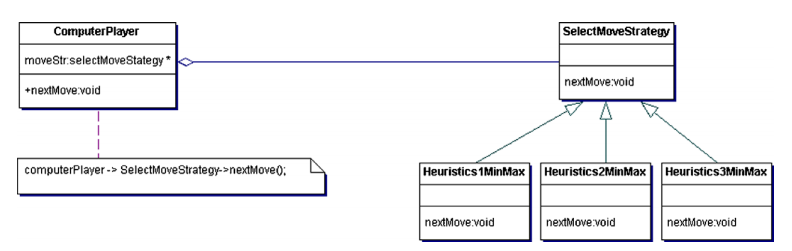
\includegraphics[width=\textwidth]{pics/strategypattern.png}
      \end{figure}

      {\bf Observer Pattern:} the observer pattern defines a one-to-many dependency between objects that when one objects changes state, all its dependants are notified and updated automatically. This can be used in a situation where a football manager game a team hires a trainer that upgrade players attributes.

      \begin{figure}[H]
        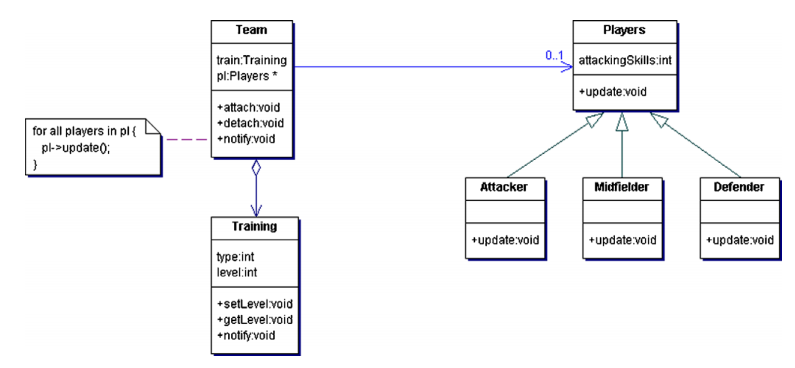
\includegraphics[width=\textwidth]{pics/observerpattern.png}
      \end{figure}

    \subsubsection*{Object-Oriented design patterns in GAME GRAPHICS}

    {\bf State Pattern:} the state pattern allows an object to alter it behaviour when its internal state change. This pattern can be used in games where an object changes the level of detail (LOD) of it apperance with respect of its distance from the camera. Feks a first person shooter, all objects of a scene should look more elegant as the main character reaches them. 

      \begin{figure}[H]
        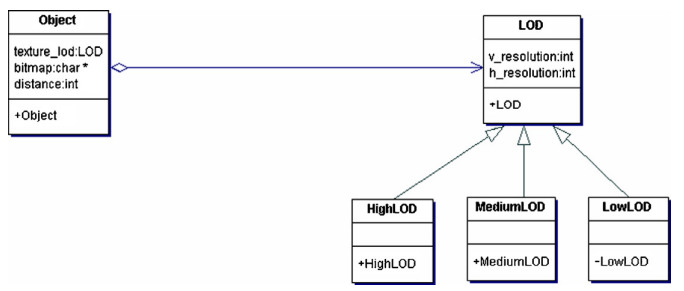
\includegraphics[width=\textwidth]{pics/statepattern.png}
      \end{figure}

    {\bf Bridge Pattern:} the bridge pattern decpuples an abstraction from its implementation so that the two can vary independently. This pattern can be used in any game with 3D objects that can be painted multiple ways. At the same time the 3D object might also vary since it can be a primitive (sphere, cube, etc) or an export from a 3D package. 

      \begin{figure}[H]
        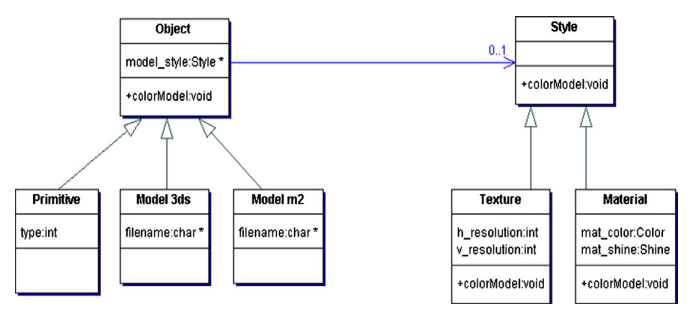
\includegraphics[width=\textwidth]{pics/bridgepattern.png}
      \end{figure}

  \section*{Evaluation}

    \subsubsection*{Software quality metrics}
    The software metrics that have been calculated can be divided into four main categories: size, complexity, coupling, and cohesion. 
    Coupling reduces the dependencies in calasses. 

      \begin{itemize}
        \item Lines of Code (LOC)
        \item Number of classes (NOC)
        \item Attribute Complexity (AC)
        \item Weighted Methods per Class 1 and 2 (WMPC1 and WMPC2)
        \item Cyclomatic Complexity (CC), number of possible paths.
        \item Coupling Factors (CF)
        \item Lack of Cohesion of Methods (LCOM)
      \end{itemize}

    \subsubsection*{Evaluation Example 1 - Cannon Smash}
    The drawback in the presented approach is that the incoming data could be recieved in three different types and according to the current type a different reading strategy should be used. In the first version the programmers used a switch statement to implement this mechanism. This code suffers from needless repitation. This code is not reuseable, because the program is not flexible enough to easily adapt the extra strategies. 

    A possible solution would be to use the strategy patten and in this way the complexity of the model will be decreased wheras the flexibility will increase. Attribute Complexity (AC) increased, Coupling decreased. Maintainable code. 

    \subsubsection*{Evaluation Example 2 - Ice Hockey Manager}
    Ice Hockey Manager is a simulation of coaching a hockey team. In the first version they used 8 design patterns. In a later version 26 design patterns was implemented, where bridge and state was two of the patterns used. 

    The state pattern represent the fact that a hockey player can either be a goalkeeper or a field player. This way, ant client of the program can create or handle a player without having to know in prior whether he is a goalkeeper or a field player. 

    The bridge pattern is used in order to provide a link between player an the player attributes interfaces so that the implementation of class player can be configured at run-time. 
    


